\documentclass[a4paper,oneside,12pt]{report}

\usepackage[utf8]{inputenc}
\usepackage[T1]{fontenc}
\usepackage[french]{babel}
\usepackage{hyperref}
\usepackage{fancyhdr}
\usepackage[official]{eurosym}
\usepackage{stageutc}

\newcommand{\cf}[1]{cf. #1}
\newcommand{\etranger}[1]{\textit{#1}}

\newcommand{\refsection}[1]{section~\ref{#1}}
\newcommand{\cfsection}[1]{\cf{\refsection{#1}}}

\newcommand{\reffigure}[1]{figure~\ref{figure:#1}}
\newcommand{\cffigure}[1]{\cf{\reffigure{#1}}}


\newcommand{\acentreon}{Centreon}
\newcommand{\alinotp}{LinOTP}
\newcommand{\aintranet}{Intranet}
\newcommand{\atypo}{Typo3}

\newcommand{\asmile}{Smile}
\newcommand{\abusys}{BU Système}

\newcommand{\ame}{Jérémy Subtil}
\newcommand{\apakou}{Patrick Kouassi}
\newcommand{\asuiveur}{Dritan Nace}
\newcommand{\amabes}{Maxime Besson}
\newcommand{\agulet}{Guilhem Lettron}




\title{TN10 -- Rapport de stage}
\subtitle{Ingénieur système et développement en environnement open source}
\author{\ame}
\date{Semestre~P11}
\keywords{open source, qualité logicielle, intégration continue, système, OTP, authentification, sécurité, supervision}

\makeatletter
\hypersetup{
	pdftitle={\@title},
	pdfauthor={\@author},
	pdfsubject={\@subtitle},
	pdfkeywords={\@keywords}
}
\makeatother

\graphicspath{{figs/}}

\geometry{headheight=15pt} % for fancyhdr


\begin{document}

\maketitle

\section*{Remerciements}

Je souhaite remercier \apakou, directeur de la \abusys, qui m'a accueilli dans son équipe chez \asmile{} et qui a suivi mon évolution au cours de ces six mois de stage.

Je remercie également mon maître de stage \agulet, ingénieur système, pour m'avoir guidé tout au
long du stage, m'avoir appris un tas de choses et m'avoir payé quelques verres.

Je voudrais aussi exprimer ma gratitude envers \amabes, expert technique système, qui m'a toujours accordé du temps pour répondre à mes questions.

Je remercie également \asuiveur, mon tuteur de stage de l'UTC, pour son soutien.

Enfin, je souhaiterais exprimer mes remerciements envers tous mes collègues titulaires et bizus\footnote{C'est ainsi que l'on surnomme les stagiaires dans la \abusys.} qui m'ont tous toujours bien accueilli parmi eux et avec qui j'ai passé d'excellents moments.


\newpage

\tableofcontents
\listoffigures
\newpage

\section*{Résumé technique}

\paragraph{}
\asmile{} est une Société de Services en Ingénierie Informatique (SSII) française, dont l'activité principale repose sur le développement web et l'intégration de solutions open source.
\asmile{} est d'ailleurs aujourd'hui considéré comme le leader français dans le domaine.
Passionné par l'écosystème de l'open source, c'est naturellement que j'ai choisi d'intégrer cette entreprise pour effectuer mon projet de fin d'études.

\paragraph{}
Mon sujet de stage initial porte sur les problématiques d'intégration continue.
Comment tester en continu la qualité d'un développement logiciel ?
Quelles sont les outils permettant de construire une offre favoriserait l'émergence de cette qualité ?

En faisant intervenir mes connaissances concernant les bonnes pratiques du génie logiciel et en développant mes compétences système, j'ai pu tester ces outils comme Jenkins, Redmine ou Selenium et participer à leur mise en place chez des clients.

\paragraph{}
En parallèle, j'ai eu l'opportunité de travailler de bout en bout sur la mise en place d'une solution d'authentification open source particulière chez un client : \alinotp.
Elle fait intervenir les OTP, ou \etranger{One-Time Passwords}, qui sont en réalité des mots de passe éphémères générés par un matériel tiers.

\paragraph{}
En outre, j'ai pu améliorer d'autant plus mes compétences en travaillant sur de l'administration système interne ou en participant à d'autres projets clients, comme la mise en place d'une plateforme de supervision avec \acentreon{} ou en intervenant en tant que support sur un projet de développement d'application web.

\paragraph{Mots-clés}
\makeatletter
\@keywords
\makeatother


\newpage

% fancyhdr
\pagestyle{fancy}
\lhead{}

\chapter{Présentation de l'entreprise}

TODO


\chapter{Déroulement du stage}

\section{Ma place au sein de la \abusys}

\paragraph{}
Passionné par l'écosystème de l'open source, c'est naturellement que j'ai choisi de postuler chez \asmile{} pour effectuer mon projet de fin d'études.
Sortant de la filière SRI de l'UTC, j'étais très intéressé de développer mes compétences système et c'est ainsi que j'ai pu intégrer la \abusys{}.

\paragraph{}
Dès mon premier entretien, j'ai défini avec \agulet{}, mon futur tuteur dans l'entreprise, le sujet principal de mon stage : nous avons choisi que je travaille sur les problématiques d'intégration continue.
En effet, à la \abusys{}, c'est une des spécialités de \agulet{}.
Il en est le référent quand il s'agit de fournir une prestation autour de ce domaine pour le compte de clients.
Pour ma part, c'est un sujet qui m'enthousiasme car il fait à la fois intervenir des connaissances en système et en qualité logicielle.
Ainsi, mon travail et ma réflexion sur l'intégration continue et ses outils sont développés dans le \refchap{pic}.

\paragraph{}
Par ailleurs, j'ai eu l'opportunité de travailler de bout en bout sur la mise en place d'une solution d'authentification open source particulière chez un client : \alinotp.
Elle fait intervenir les OTP, ou \etranger{One-Time Passwords}, qui sont en réalité des mots de passe éphémères générés par un matériel tiers.

Cette mission s'est déroulée sur la fin de mon stage, et j'ai alors eu l'opportunité de réaliser un véritable travail d'ingénieur système au même titre que mes collègues titulaires.
Elle est décrite en détail dans le  \refchap{linotp}.

\paragraph{}
En outre, j'ai eu l'occasion de travailler sur une multitude d'autres projets de taille plus ou moins importante :

\begin{itemize}
	\item mettre en place chez un client une solution de supervision \acentreon{} (\cfchap{centreon}) ;
	\item apporter un soutien au développement d'un projet client en retard pour \abt{} (développement avec le framework PHP Symfony et le framework JavaScript ExtJS) ;
	\item mettre en place une plateforme web de visioconférence pour \asmile{} avec la solution libre BigBlueButton ;
	\item auditer le code du logiciel libre Linbox-Converter pour le compte de Renault, qui permet de convertir des documents Microsoft Office vers d'autres formats ;
	\item chiffrer des projets système dans le cadre des processus d'avant-vente de \asmile.
\end{itemize}

\paragraph{}
Aussi, j'ai régulièrement eu à apporter un support d'administration système dit \emph{support projet} aux projets des différentes BU de développement de \asmile{}.
Ce support se concrétise par un certain nombre de tâches récurrentes :

\begin{itemize}
	\item la création d'environnements virtuels\footnote{La virtualisation consiste à faire fonctionner sur un seul ordinateur plusieurs systèmes d'exploitation comme s'ils fonctionnaient sur des ordinateurs distincts. On appelle serveur privé virtuel (\etranger{Virtual Private Server} ou VPS) ou encore environnement virtuel (\etranger{Virtual Environment} ou VE) ces ordinateurs virtuels.~\cite{virtualisation}} sur des serveurs de façon à pouvoir mettre en recette des projets web ;
	\item la migration d'environnements virtuels sur des serveurs différents ;
	\item la création de domaines via des serveur DNS\footnote{Le \etranger{Domain Name System} (ou DNS, système de noms de domaine) est un service permettant d'établir une correspondance entre une adresse IP et un nom de domaine et, plus généralement, de trouver une information à partir d'un nom de domaine.~\cite{dns}} Bind pour accéder à ces environnements de recette ;
	\item la configuration de serveurs HTTP\footnote{L'\etranger{HyperText Transfer Protocol}, plus connu sous l'abréviation HTTP, est un protocole de communication client-serveur développé pour le \etranger{World Wide Web}. Les clients HTTP les plus connus sont les navigateurs Web permettant à un utilisateur d'accéder à un serveur contenant les données. Ces clients se connectent à des serveurs HTTP tels qu'Apache ou IIS de Microsoft.~\cite{http}} Apache ;
	\item la création de dépôts de code source Subversion (\cfsection{pic-source}) ;
	\item la création et le dépannage de bases de données MySQL ou Oracle ;
	\item la création de comptes FTP\footnote{Le \etranger{File Transfer Protocol} (protocole de transfert de fichiers), ou FTP, est un protocole de communication destiné à l'échange informatique de fichiers sur un réseau TCP/IP. Il permet, depuis un ordinateur, de copier des fichiers vers un autre ordinateur du réseau, d'alimenter un site web, ou encore de supprimer ou de modifier des fichiers sur cet ordinateur.~\cite{ftp}}.
\end{itemize}

\paragraph{}
Enfin, j'ai pu commencer certains travaux qui n'ont pas pu aboutir pour diverses raisons.
Ceux-ci sont décrits brièvement en fin de rapport à la \refsection{avortes}.



\section{Planning effectif}

\paragraph{Février}
\begin{itemize}
	\item Support projet
	\item Mise en place d'un serveur de base de données Oracle
	\item Auto-formation sur la réplication de bases de données MySQL
	\item Auto-formation sur les outils Jenkins et Selenium
	\item Travail sur l'offre \og plateformes d'intégration continue \fg{} (PIC)
\end{itemize}

\paragraph{Mars}
\begin{itemize}
	\item Support projet
	\item Tentative de mise en place d'OpenMCU en interne
	\item Auto-formation sur l'ESB \apetals{}
	\item Développement sur le projet Abitbol
\end{itemize}

\paragraph{Avril}
\begin{itemize}
	\item Support projet
	\item Développement sur le projet Abitbol
	\item Développement Redmine
	\item Audit de code Linbox-Converter pour Renault
	\item Projet \acentreon{} pour \adacast{}
	\item Travail sur l'offre PIC
\end{itemize}

\paragraph{Mai}
\begin{itemize}
	\item Support projet
	\item Mise en place de BigBlueButton en interne
	\item Projet LinOTP pour la CNIL
	\item Travail sur l'offre PIC
\end{itemize}

\paragraph{Juin}
\begin{itemize}
	\item Support projet
	\item Fin du projet LinOTP pour la CNIL
	\item Rédaction d'une ébauche de livre blanc sur l'offre PIC
	\item Soutien au développement du projet de développement pour \abt{}
\end{itemize}

\paragraph{Juillet}
\begin{itemize}
	\item Soutien au développement du projet de développement pour \abt{}
\end{itemize}


\chapter{L'offre \og plateformes d'intégration continue \fg}
\label{section:pic}

\paragraph{}
Quand on sait que 70\% des projets informatiques ne respectent pas le planning initial ou se transforment en échecs~\cite{echec}, on cherche par tous les moyens à réduire les facteurs responsables.
Le manque de qualité logicielle et de suivi de projet en font évidemment parti.
Alors que ces domaines étaient encore un marché de niche il y a quelques temps de cela, aujourd'hui, de plus en plus de clients et de DSI\footnote{Directions de Services Informatiques} commencent à s'en préoccuper et à remettre en cause les méthodes classiques de gestion de projets informatiques.
C'est aussi l'occasion de tenter de pérenniser les développements qui au fil du temps perdent toujours plus en maintenabilité.

\paragraph{}
La qualité logicielle et le suivi de projets informatiques deviennent donc un véritable enjeu actuel.
Les entreprises doivent alors se doter de nouveaux process et de nouveaux outils. 
Elles peuvent les acquérir en faisant notamment appel à des prestations de conseil dans le domaine, qui font entre autres intervenir des notions de gestion de projet et de bonnes pratiques en terme de génie logiciel.
Au-delà de ça, les nouveaux outils doivent être mis en place et intégrés aux infrastructures systèmes existantes.

\paragraph{}
C'est ainsi que la \abusys{} de \asmile, sous l'impulsion de \agulet, s'est positionnée sur ce marché.
Une offre open source a été construite pour répondre au besoin de A à Z, de l'installation des outils au conseil sur leur utilisation, en passant par leur configuration personnalisée.


\section{Intérêt des méthodes agiles}

\paragraph{}
Les méthodes agiles sont très répandues dans les communautés du logiciel libre.
Les programmes y sont souvent développés en en suivant les principes.
Raison de plus pour que \asmile{}, leader sur le marché de l'open source, fasse la promotion de l'agilité après des entreprises.


\paragraph{}
Les méthodes agiles partent du constat que les spécifications initiales du client sont souvent \og volatiles \fg, dans le sens où elles évoluent relativement vite dans le temps et qu'elles souffrent régulièrement d'imprécision.
Les méthodes lourdes classique de développement impliquant spécifications, réalisation puis recette par le client se révèlent donc inadaptées.
Au contraire, il faut privilégier des cycles de développement courts qui apportent la flexibilité nécessaire pour pouvoir corriger rapidement à coût moindre les éventuelles erreurs de spécification ou de conception.

L'organisation du développement épouse alors deux aspects :

\begin{itemize}
	\item le côté itératif, car le logiciel est créé sur plusieurs cycles d'une durée relativement courte ;
	\item l'aspect incrémental, car chaque nouveau cycle améliore les fonctionnalités du précédent.
\end{itemize}


\paragraph{}
En outre, le Manifeste Agile~\cite{agile}, considéré comme l'acte généralisateur des méthodes agiles, invite à adopter un certain nombre de valeurs :

\begin{itemize}
	\item il faut privilégier les personnes et les interactions plutôt que de suivre aveuglément des procédures et d'être dirigé par ses outils ;
	\item la création régulière de jalons fonctionnels est une priorité pour garder cons\-tam\-ment à l'idée ce qu'est et ce que va être le produit final ;
	\item la clé est la collaboration étroite avec le client, alors que l'on a traditionnellement tendance à respecter un contrat et à suivre des spécifications initiales ;
	\item le client et le prestataire réalisateur doivent tous deux être flexible et accepter le changement.
\end{itemize}


\paragraph{}
Les méthodes agiles sont parfois difficiles à mettre en place car elles sont souvent en rupture avec les processus existants de l'entreprise.
De plus, la flexibilité requise peut être confondue avec un défaut d'organisation, ce qui amène inévitablement à des résultats catastrophiques.
Au contraire, de bons outils adaptés sont nécessaires pour effectuer un vrai suivi du projet.
Ils doivent permettre de tracer de façon transparente les changements et d'améliorer la communication entre les différents acteurs du projet.



\section{La gestion de projet agile}

\subsubsection{Outil : Redmine}

\subsubsection{Outil : JIRA}

\subsubsection{Mission : Formation JIRA chez Rexel}

\subsubsection{Mission : Développement Redmine}

- Développement de plugins

- Contribution au core



\section{Gestion de versions du code source}
\label{section:pic-source}

\subsection{Outils}

\subsubsection{Subversion}

\subsubsection{Git}

\subsection{Missions}

\subsubsection{Formation Subversion chez Rexel}

\subsubsection{Synchronisation de mirroirs SVN pour Rexel}

\subsubsection{Plan de formation Git}



\section{Tests des applications}

Tester l'application est une condition nécessaire si l'on veut s'assurer de sa qualité.
Les tests manuels par les développeurs ou les utilisateurs sont loin d'être suffisants : il existe bien trop de cas à vérifier.
Pour répondre à ce problème d'exhaustivité, il est possible de mettre en place des tests automatiques et programmables.
Aussi, on peut distinguer deux types de tests : les tests \emph{unitaires} et les tests \emph{fonctionnels}.



\subsection{Tests unitaires}

Pour expliquer ce qu'est ce premier type de tests, je m'en réfère à l'excellent article Wikipédia à ce sujet.~\cite{unit}

\begin{quotation}
Le test unitaire est un procédé permettant de s'assurer du fonctionnement correct d'une partie déterminée d'un logiciel ou d'une portion d'un programme (appelée \og unité \fg{} ou \og module \fg).

On écrit un test pour confronter une réalisation à sa spécification. Le test définit un critère d'arrêt (état ou sorties à l'issue de l'exécution) et permet de statuer sur le succès ou sur l'échec d'une vérification.
Grâce à la spécification, on est en mesure de faire correspondre un état d'entrée donné à un résultat ou à une sortie.
Le test permet de vérifier que la relation d'entrée/sortie donnée par la spécification est bel et bien réalisée.

Il s'agit pour le programmeur de tester un module, indépendamment du reste du programme, ceci afin de s'assurer qu'il répond aux spécifications fonctionnelles et qu'il fonctionne correctement en toutes circonstances.
Cette vérification est considérée comme essentielle, en particulier dans les applications critiques.
Elle s'accompagne couramment d'une vérification de la couverture de code (évaluation de la couverture structurelle), qui consiste à s'assurer que le test conduit à exécuter l'ensemble (ou une fraction déterminée) des instructions présentes dans le code à tester.

L'ensemble des tests unitaires doit être rejoué après une modification du code afin de vérifier qu'il n'y a pas de régressions (l'apparition de nouveaux dysfonctionnements).
\end{quotation}



\subsection{Tests fonctionnels}

Les tests fonctionnels diffèrent des tests unitaires du point de vue qu'ils vérifient les fonctionnalités de l'application.
Leur portée s'éloigne ainsi du code et devient globale à l'application.

Au niveau d'un site web, par exemple, un test fonctionnel consiste à naviguer à l'intérieur, en cliquant sur des liens, en remplissant des formulaires, ou encore en vérifiant si divers éléments d'une page sont bien présents.

Ce type de test prend tout son intérêt quand il s'agit de tester un cas d'utilisation typique d'une application par ses utilisateurs finaux.
En reproduisant un ensemble significatif des scénarios utilisateurs sous forme de tests fonctionnels, on peut alors s'assurer du bon fonctionnement global du programme, quels que soient les changement de code entrepris.



\subsection{Outils}

\subsubsection{Librairies de tests unitaires}

\paragraph{}
Chaque langage de programmation dispose de sa librairie pour rédiger des tests unitaires, si ce n'est plus.
Par exemple, on va trouver JUnit pour Java, PHPUnit ou Lime pour PHP, CppTest pour C++, etc.

\paragraph{}
La façon de rédiger des tests est souvent la même malgré les différences entre langages de programmation.
Pour une fonction, ce processus est répété pour chaque ensemble de paramètres d'entrée à tester :

\begin{enumerate}
	\item le contexte d'exécution est défini à travers des définition de variable est des appels de fonctions ;
	\item la fonction à tester unitairement est appelée, avec en entrée des paramètres choisis pour être des cas classiques ou des cas limites ;
	\item le retour de la fonction (voire même le déclenchement d'exception) est comparé à un résultat attendu issu des spécifications.
\end{enumerate}

Ainsi, chaque fonction à tester est exécutée plusieurs fois de suite avec des paramètres d'entrée différents afin de bien couvrir tous les cas.



\subsubsection{Selenium}

\paragraph{}
Selenium est un outil de tests fonctionnels pour les sites web.
Disponible sous la forme d'une extension pour le navigateur web Firefox, il enregistre l'enchaînement des liens cliqués pour naviguer de page en page.
Quand le test est joué, si une page du scénario ne s'affiche pas, on considère que c'est un échec.

Un autre test souvent utilisé est la vérification de la présence d'un texte sur une page.
C'est très pratique dans le cas où l'on veut vérifier la présence ou non d'erreurs après la soumission d'un formulaire, par exemple.

Enfin, le jeu de tests peut être sauvé dans un fichier afin de pouvoir être rejoué ultérieurement.

\paragraph{}
La \reffigure{pic-tests:selenium} montre une capture d'écran de Selenium.

\begin{figure}
	\centering
	\includegraphics[width=7cm]{pic/selenium-ide}
	\caption{Selenium en action}
	\label{figure:pic-tests:selenium}
\end{figure}



\subsection{Missions}

\subsubsection{Formation Selenium chez Spir}

\paragraph{}
Spir est un éditeur de journaux de petites annonces qui édite aujourd'hui des sites \ainternet{} comme Top Annonces ou Logic Immo.
Pour améliorer son processus qualité, le client désire s'équiper d'un outil permettant de jouer automatiquement des tests fonctionnels.

\paragraph{}
Je me suis alors rendu dans leurs locaux avec \agulet{} pour leur présenter l'outil Selenium.
C'est une formation que j'ai préparée en amont moi-même et que nous avons présenté au client en duo.



\section{Intégration continue}

\subsection{Outils}

\subsubsection{Hudson/Jenkins}

\subsection{Missions}

\subsubsection{paramétrage de la PIC de Spir}

\subsubsection{Formation Jenkins chez Spir}



\section{Bilan}

\paragraph{}
Finalement, \asmile{} fournit une offre complète d'intégration système autour des méthodes agiles et de l'intégration continue.
Le client peut suivre son projet avec Redmine, manipuler son code source avec Subversion tout en conservant un historique de l'ensemble des changements effectués, et enfin tester son application en continu avec Jenkins.
Il est accompagné par les ingénieurs système de \asmile{} qui peuvent lui proposer une prestation de conseil.

\paragraph{}
La \reffigure{pic:bilan} offre une vue d'ensemble de l'offre.

\begin{figure}
	\centering
	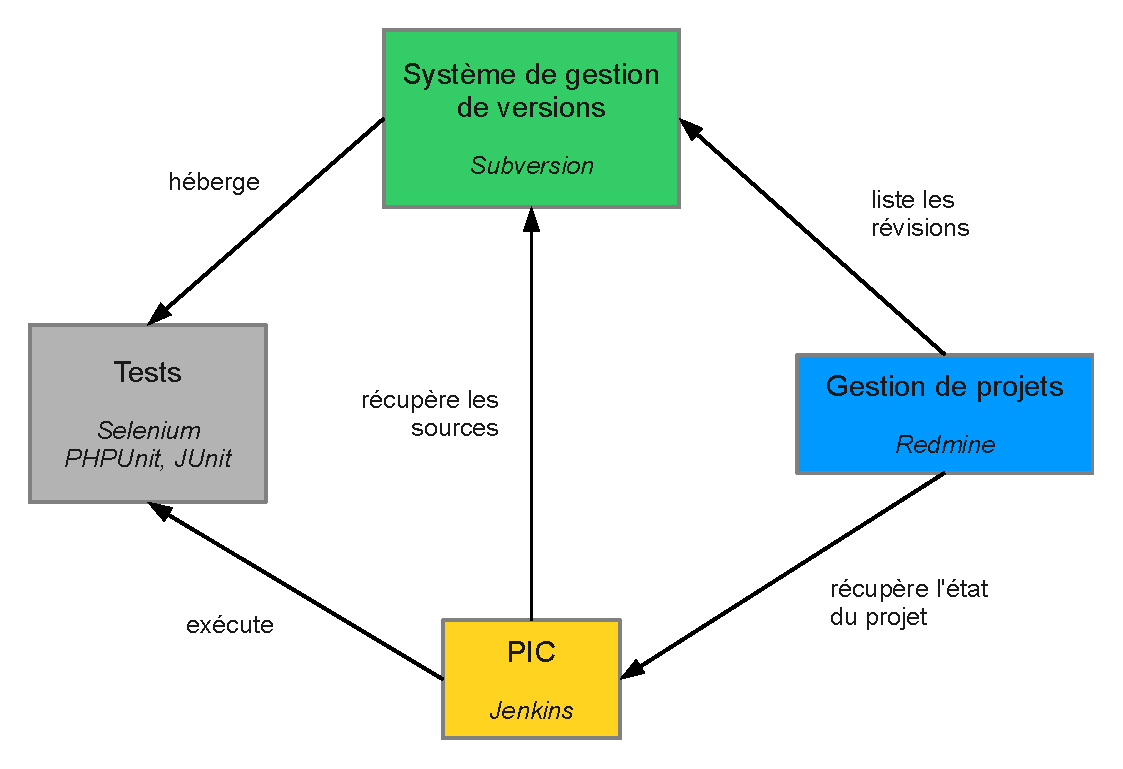
\includegraphics[width=14cm]{pic/bilan}
	\caption{Vue d'ensemble de l'offre \og Plateformes d'intégration continue \fg}
	\label{figure:pic:bilan}
\end{figure}




\section{Mise en place d'une solution \alinotp{}}

TODO


\section{Mise en place d'une solution \acentreon{}}

\subsection{La solution \acentreon}

\paragraph{}
\acentreon{} est une plateforme open source de supervision, c'est-à-dire de surveillance du bon fonctionnement d'une infrastructure système.

\paragraph{Principe de la supervision}
De façon classique, on surveille toutes les informations relatives au matériel (température, pannes\ldots) et au système (charge serveur, utilisation de la mémoire et du processeur\ldots) des serveurs d'un parc.
Généralement, on supervise également tous les services applicatifs (serveurs web, serveurs FTP, serveurs de base de données\ldots) qui y sont hébergées.

Ainsi, les administrateurs système peuvent savoir en temps réel quels sont les services et les machines qui sont fonctionnels ou hors-service.
Très souvent, des alertes leurs sont envoyées pour les prévenir d'une rupture de service.
Ces alertes peuvent prendre la forme d'e-mails mais aussi de SMS ou de messages envoyés par messagerie instantanée.

\paragraph{\anagios}
La solution \acentreon{} repose sur \anagios{} pour effectuer toutes les opérations de surveillance, de reporting et de d'alerte.
Par défaut, \anagios{} propose un certain nombre de possibilités que ce soit pour superviser les ressources des serveurs, les services actifs en consultant un port\footnote{Correspondant à la couche de transport du modèle OSI, la notion de port logiciel permet, sur un ordinateur donné, de distinguer différents interlocuteurs. Ces interlocuteurs sont des programmes informatiques qui, selon les cas, écoutent ou émettent des informations sur ces ports. Un port est distingué par son numéro.~\cite{port}} donné ou en interrogeant les machines via le protocole SNMP\footnote{SNMP (pour \etranger{Simple Network Management Protocol}) est un protocole de communication qui permet aux administrateurs réseau de gérer les équipements du réseau, de superviser et de diagnostiquer des problèmes réseaux et matériels à distance.~\cite{snmp}}.

Les possibilités de supervision sont infinies car \anagios{} est doté d'un système de plugins très efficace.
En effet, ces plugins sont de simples programmes exécutables via la ligne de commande, auxquels on passe en paramètre des options de configuration et qui retournent un entier.
On peut donc les développer dans n'importe quel langage de programmation.
C'est la valeur du code retour qui précise si le test effectué par le plugin est passé ou non :

\begin{description}
	\item[0 OK] le test est passé ;
	\item[1 WARNING] le seuil d'alerte est dépassé ;
	\item[2 CRITICAL] le service a un problème ;
	\item[3 UNKNOWN] il est impossible de connaître l'état du service.
\end{description}

Ces différents niveaux, en plus de permettre le déclenchement d'alertes, sont facilement distinguables sur l'interface web de \anagios{} via un code couleur (\cffigure{centreon:nagios}).

Enfin, il est possible de lancer des actions de surveillance à distance via le protocole NRPE (\etranger{Nagios Remote Plugin Executor}).
En effet, celui-ci permet de lancer n'importe quel plugin \anagios{}, si celui-ci est bien installé sur la machine interrogée.
Les informations transitent entre le serveur \anagios{} et les machines surveillées via un tunnel SSL\footnote{SSL (pour \etranger{Secure Sockets Layer}) est un protocole de sécurisation des échanges sur Internet.~\cite{tls}} sécurisé.

\begin{figure}
	\centering
	\includegraphics[width=12cm]{centreon/nagios-notifications}
	\caption{Historique des notifications sur Nagios}
	\label{figure:centreon:nagios}
\end{figure}

\paragraph{\acentreon}
Le principal avantage de ce complément à \anagios{} est de fournir une interface graphique web efficace, claire et plus simple à appréhender (\cffigure{centreon:centreon}).

Il ajoute entre autres une gestion fine des utilisateurs, des plugins \anagios{} supplémentaires, des représentations graphiques élaborées, des possibilités d'architecture distribuée, etc.

\begin{figure}
	\centering
	\includegraphics[width=12cm]{centreon/centreon-status}
	\caption{État en temps réel des services sur \acentreon{}}
	\label{figure:centreon:centreon}
\end{figure}


\subsection{Contexte de la mission}

\paragraph{}
Le client de \asmile{} pour cette mission était \adacast.
C'est une relativement jeune startup présente en France et aux États-Unis.
Son concept est de fournir une plateforme de diffusion multimédia à la demande, en live ou non, performante et simple à utiliser.
Ainsi, ses clients fournissent leurs flux audio ou vidéo et c'est \adacast{} qui se charge de les transformer dans le bon format et les diffuser tout en supportant les éventuels pics d'audience.
\adacast{} propose également différentes façon de monétiser les diffusions, que ce soit par la publicité, par un paiement à la vue ou au forfait.

\paragraph{}
Dans ce contexte, \adacast{} souhaite s'équiper d'une solution de supervision pour surveiller en temps réel son parc de serveurs.
En effet, jusqu'ici, les vérifications de disponibilité de ses services étaient relativement primaires alors que son offre, son nombre de clients et ses enjeux deviennent de plus en plus importants.
Toute rupture de service devient vite critique et doit être prise en charge dans les plus brefs délais.
Il s'agit aussi pour \adacast{} de faire preuve de professionnalisme envers ses clients en dépannant les problèmes avant de recevoir tout coup de fil de plainte.

\paragraph{}
Chez \asmile{}, \asegir{} est le spécialiste de la solution de supervision \acentreon{}.
Je l'ai donc suivi lors de son intervention chez \adacast{} pour apprendre à maîtriser cette technologie.
Nous avons travaillé ensemble la première journée durant laquelle il m'a formé, et j'ai pu terminer la mission seul le lendemain.
\asegir{} est ensuite intervenu à nouveau pour fournir une documentation et former les utilisateurs.


\subsection{Notre démarche}

\paragraph{}
Pour réduire les coûts et limiter le temps d'intervention, \adacast{} n'a commandé que l'installation de la solution \acentreon{} et la supervision de deux serveurs.
La supervision des autres serveurs serait alors effectuée par ses ressources internes.

\paragraph{}
Pour installer la plateforme \acentreon{}, nous avons demandé à notre interlocuteur de nous fournir un serveur indépendant.
En effet, il est important que la solution de supervision soit sur un serveur qui soit indépendant des serveurs à surveiller.
L'intérêt est à la fois de séparer les services et de ne pas être soumis aux même pannes que ce qui doit être supervisé.

Le client a choisi de commander un serveur à bas coût -- de l'ordre de 20\euro~HT par mois -- chez un hébergeur externe.
Une telle configuration minimaliste est suffisante pour le besoin car peu d'utilisateurs vont consulter la plateforme \acentreon{} et le trafic relatif à l'échange de données de surveillance est limité.

\asegir{} m'a alors montré comment installer \acentreon{} sur un système \alinux{} Ubuntu Server.

\paragraph{}
Nous sommes ensuite passés à la partie la plus intéressante de l'intervention, c'est-à-dire la configuration de la solution en fonction des besoins du client.
Pour cela, des démons NRPE ont été installés sur chaque serveur à superviser.
Nous avons alors mis en place un certain nombre de plugins pour couvrir le périmètre attendu, qui inclut entre autres :

\begin{itemize}
	\item la surveillance des ressources des machines (consommation processeur et mémoire, charge serveur, espace disque disponible) ;
	\item le fonctionnement du RAID matériel ;
	\item la surveillance de la disponibilité de ses services (HTTP, MySQL, FTP, SSH, etc.) ;
	\item la surveillance des métriques relatives à l'utilisation de leur base de données MySQL.
\end{itemize}

\paragraph{}
Enfin, une vue d'ensemble de l'architecture mise en place est illustrée en \reffigure{centreon:archi}.

\begin{figure}
	\centering
	\includegraphics[width=12cm]{centreon/archi}
	\caption{Architecture de supervision mise en place chez \adacast{}}
	\label{figure:centreon:archi}
\end{figure}


\chapter{Le support projet}
\label{section:support}

TODO


\chapter{Bilan personnel}

\paragraph{}
J'ai beaucoup apprécié ce stage TN10 chez \asmile.
Le travail sur l'offre PIC avec mon maître de stage \agulet{} était très enrichissant, j'ai vraiment pu pousser les connaissances basiques que j'avais dans le domaine.
Notamment, j'ai pu acquérir une vision globale de l'offre d'intégration qui pouvait être proposée autour des concepts des méthodes agiles et de l'intégration continue.
Conseil, mise en place de processus de qualité et formation constituent la valeur ajoutée que peut apporter l'ingénieur.

Toutefois, je reste un peu déçu de ne pas avoir été confronté à un gros projet client de A à Z dans le domaine.

\paragraph{}
J'ai aussi beaucoup appris de ma mission d'intégration de solution OTP.
En contact direct avec le client et l'éditeur, j'ai à la fois pu mêler déploiement technique et gestion de projet.
À l'issue de ma formation à l'UTC et de ces six mois de stage de fin d'étude, c'est grâce à ces savoir-faire que je suis aujourd'hui devenu un ingénieur. 

\paragraph{}
Enfin, grâce aux plus petites missions système et au tâches de support projet, j'ai pu améliorer mes compétences techniques dans le domaine de l'administration système.

\paragraph{}
Malgré tous ces points positifs, j'ai décidé de ne pas travailler dans le domaine du système mais plutôt dans celui du développement.
Je pense y avoir un véritable potentiel que je prendrai plaisir à cultiver.
Le métier d'Ingénieur Études et Développement est donc un poste qui est plus en adéquation avec mes passions personnelles.

Mes compétences en ingénierie système restent néanmoins un véritable atout.
Cette compréhension globale des systèmes d'information, de la création logicielle à l'exploitation en passant par les mises en production, est une capacité que je pourrai mettre en avant dans ma carrière professionnelle.


\newpage

\bibliographystyle{plain}
\addcontentsline{toc}{chapter}{Bibliographie}
\bibliography{biblio}
\newpage

\appendix

\chapter{Captures d'écran de Redmine}
\label{annexe:redmine}

TODO


\chapter{Captures d'écran de JIRA}
\label{annexe:jira}

TODO


\chapter{Captures d'écran de Jenkins}
\label{annexe:jenkins}

TODO



\end{document}

